\subsection{Runtime Adaptation}
\label{sec:runtime}

\begin{figure}
  \centering
  % \resizebox{\columnwidth}{!}{
  %   \begin{tikzpicture}
  %
  % Define basic styles
  %
  % Node
  \tikzstyle{module} = [draw, very thick, rounded corners,
  fill=white, minimum height=2.5em, inner sep=0.5em,
  rectangle, font={\bfseries}, align=center]
  \tikzstyle{cmodule} = [module, fill=black!20]

  % Edge
  \tikzstyle{stateEdgePortion} = [black, thick];
  \tikzstyle{dataEdge} = [stateEdgePortion, ->];
  \tikzstyle{controlEdgePartial} = [stateEdgePortion, dashed];
  \tikzstyle{controlEdge} = [controlEdgePartial, ->];
  \tikzstyle{controlDoubleEdge} = [controlEdgePartial, <->];
  \tikzstyle{edgeLabel} = [pos=0.5, text centered, font={\itshape}];

  \node[name=client, draw, very thick, fill=white,
  double copy shadow={shadow xshift=2pt, shadow yshift=-2pt, fill=white, draw},
  text height=13em, text width=31.5em] {};

  \node[name=server, draw, very thick, fill=white, draw,
  right=of client.north east, anchor=north west, xshift=1em,
  text height=7em, text width=12.5em] {};

  \node[module, name=source, below right=of client.north west,
  xshift=-1.5em, yshift=1.5em] {Source};
  \node[module, name=transform, right of=source, xshift=3.5em] {Transform};
  \node[cmodule, name=degrade, right of=transform, xshift=3.7em] {Degrade};
  \node[cmodule, name=queue, right of=degrade, xshift=3em] {Queue};
  \node[cmodule, name=socket, right of=queue, xshift=3em, text width=3em] {Socket};
  \node[cmodule, name=receiver, right of=socket, xshift=7em] {Receiver};
  \node[module, name=analytics, right of=receiver, xshift=3em] {Analytics};

  \node[cmodule, name=cc, at=($(queue)!0.5!(socket)$), yshift=-6em]
  {Congestion\\Controller};

  \draw ($(source.east)$) edge[dataEdge] ($(transform.west)$);
  \draw ($(transform.east)$) edge[dataEdge] ($(degrade.west)$);
  \draw ($(degrade.east)$) edge[dataEdge] ($(queue.west)$);
  \draw ($(queue.east)$) edge[dataEdge] ($(socket.west)$);
  \draw ($(socket.east)$) edge[dataEdge] node[edgeLabel, yshift=0.6em] {data}
  ($(receiver.west)$);
  \draw ($(receiver.east)$) edge[dataEdge] ($(analytics.west)$);

  %% Control path
  \draw let
  \p1 = ($(cc.center)$), \p2 = ($(degrade.center)$)
  in ($(cc.west)$) edge[controlEdgePartial] (\x2, \y1)
  (\x2, \y1) edge[controlEdge] ($(degrade.south)$);

  \draw let
  \p1 = ($(queue.south)$), \p2 = ($(cc.north)$)
  in ($(\x1, \y1) + (1em,0)$) edge[controlEdge] ($(\x1, \y2) + (1em,0)$);

  \draw let
  \p1 = ($(socket.south)$), \p2 = ($(cc.north)$)
  in ($(\x1, \y1) + (-1em,0)$) edge[controlDoubleEdge] ($(\x1, \y2) + (-1em,0)$);

  \node[name=clientlabel, above right=of client.south west, xshift=-2em, yshift=-2em] {Edge (Client)};
  \node[name=clientlabel, above left=of server.south east, xshift=2em, yshift=-2em] {Server};

  %%
  %% Legend
  %%
  \node[name=datalegend, below=1.5em of server.south west, xshift=2em]
  {\small Data Plane};
  \draw ($(datalegend.west) + (-2em, 0)$) edge[dataEdge]
  ($(datalegend.west) + (-0.5em, 0)$);

  \node[name=controllegend, below=2.5em of datalegend.west, anchor=west]
  {\small Control Plane};
  \draw ($(controllegend.west) + (-2em, 0)$) edge[controlEdge]
  ($(controllegend.west) + (-0.5em, 0)$);

  \node[name=applegend, right=3em of datalegend.east]
  {\small Application Logic};
  \node[module, name=applegendbox, left=0.1em of applegend, text width=0.3em,
  minimum height=0em] {};

  \node[name=syslegend, below=2.5em of applegend.west, anchor=west]
  {\small Runtime};
  \node[cmodule, name=syslegendbox, left=0.1em of syslegend, text width=0.3em,
  minimum size=0em] {};

\end{tikzpicture}

%%% Local Variables:
%%% mode: latex
%%% TeX-master: "sosp17"
%%% End:

  % }
  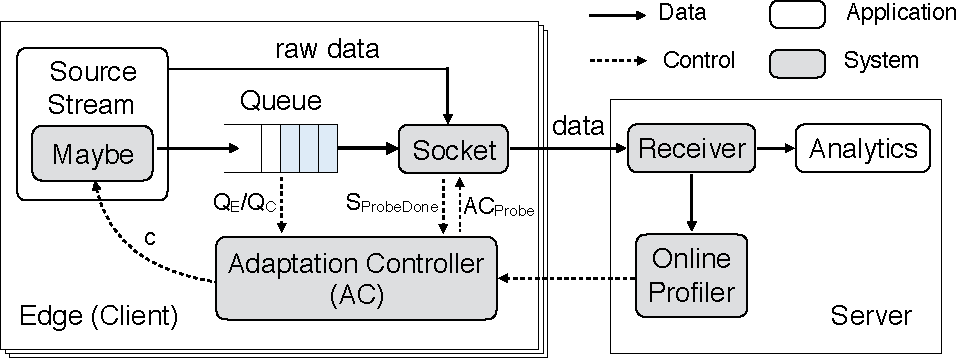
\includegraphics[width=\linewidth]{figures/runtime-adaptation.pdf}
  \caption{Runtime adaptation system architecture.}
  \label{fig:runtime}
\end{figure}

\begin{figure}
  \centering
  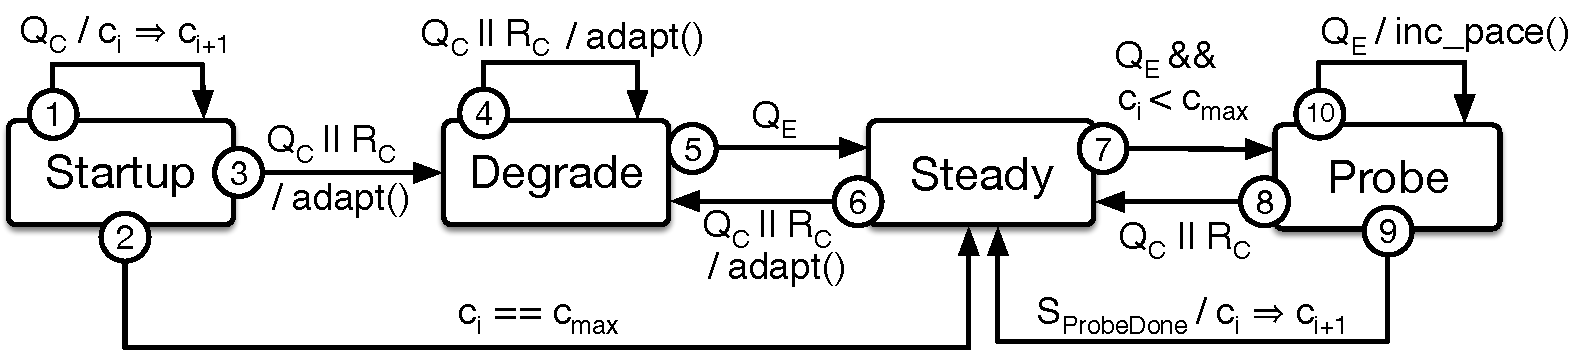
\includegraphics[width=\columnwidth]{figures/cc.pdf}
  \caption{The Adaptation Algorithm and an illustration of one possible trace.}
  \label{fig:cc}
\end{figure}

At runtime, \sysname{} creates additional modules and controls to facillitate
the runtime adaptation (\autoref{fig:runtime}).

The source stream has a \texttt{Maybe} module derived from \maybe{} that allows
the controller to \textit{update} the level of degradation. Data generated by
the source is then enqueued to a \texttt{Queue} module and subsequently dequeued
by \texttt{Socket}. When the source's data generation rate exceeds the socket's
departure rate, the queue grows. At this time, adaptation controller (AC) starts
regulating the source stream by changing the configuration. We denote the
current configuration is $c_i$. The AC's algorithm (a state machine
\autoref{fig:cc}) is described as below:

\para{Startup: rapid growth.} When the application starts up, it performs its
first and most rapid rate increase. Upon each \texttt{Q.NoQueue} message, it
advances the configuration from $c_i$ to $c_{i+1}$, increasing the data rate
discretely. The growth stops if it receives \texttt{Q.Congestion} (turning into
\texttt{Degrade} state) or $c_{i+1} == c_{max}$ (entering \texttt{Steady}
state).

\para{Degrade: reacting to congestion.} At this state, there are queued objects
hurting the application latency. AC queries the current delivery rate $R$ from
the \texttt{Socket} and \textit{update} the \texttt{Degrade} module with a
configuration $c_i$ such that $B(c_i) < \alpha R$ ($\alpha \in (0, 1)$). A
smaller $\alpha$ allows a quicker drain of the queue. After there is no more
queued objects, AC receives \texttt{Q.NoQueue} signal and enters \texttt{Steady}
state.

\para{Steady: achieving low latency delivery.} Applications achieve low latency
by spending most of its time in this \texttt{Steady} state. If the network
condition changes and the delivery bandwidth is not sufficient, the queue's
growth will reflect it and \texttt{Q.Congestion} signal will change the state to
\texttt{Degrade}. In \texttt{Steady} state, if the application is running at
maximal configuration $c_{max}$, then it will stay in this state; if current
$c_i < c_{max}$, AC will enter \texttt{Probe} state to check if there is more
available bandwidth.

\para{Probe: more bandwidth for a higher accuracy.} During the probe, the
\texttt{Socket} will send additional traffic and update the bandwidth
estimation. Instead of directly advance $c_i$, which could lead to queue and
drastic latency increase, the probing sends \textit{additional} traffic so that
the rate can be controlled in a finer granularity. If the application is
cofnigured to run online profiling, \sysname{} sends raw data as the additional
traffic; otherwise, dummy data is sent for probing. AC leaves probing state
under two conditions: (1) the available bandwith $R$ is large enough for the
next configuration $B(c_{i+1}) < R$ (\texttt{S.ProbeDone}); (2) objects are
queued (\texttt{Q.Congestion}) due to probing.

If online profiling is enabled, \texttt{Receiver} at the server side will
extract raw data and send it to online profiler. The newly-learned model is then
fed back to AC to update the profile for subsequent adaptation.

% \begin{figure}
%   \centering
%   \resizebox{\columnwidth}{!}{
%     \begin{tikzpicture}[
  state/.style = { draw, very thick, fill=white, rounded corners=1em,
    minimum height=3em, minimum width=7em, node distance=7em, font={\bfseries},
    align=center },
  edge portion/.style = { black, thick },
  transition/.style = { edge portion, -> },
  algorithm/.style = { draw, thin, fill=white },
  ]

  \node [state] (startup) {
    STARTUP };
  \node [state] (congestion) [right=of startup] {CONGESTION};
  \draw [transition] (startup) -- (congestion)
  node [midway, auto] {Q.Congestion};

  \node [state] (steady) [below=of congestion] {STEADY};

  \draw [transition] ($(congestion.south west)!0.4!(congestion.south east)$)
  to node[midway, sloped, below] {Q.NoQueue}
  ($(steady.north west)!0.4!(steady.north east)$);

  \draw [transition] ($(steady.north west)!0.6!(steady.north east)$)
  to node[midway, sloped, below] {Q.Congestion}
  ($(congestion.south west)!0.6!(congestion.south east)$);

  \node [state] (probe) [left=of steady] {PROBE};

  \draw [transition] ($(steady.south west)!0.6!(steady.north west)$)
  -- ($(probe.south east)!0.6!(probe.north east)$)
  node[midway, auto, swap] {Q.Probe};

  \draw [transition, <-] ($(steady.south west)!0.4!(steady.north west)$)
  -- ($(probe.south east)!0.4!(probe.north east)$)
  node[midway, auto, align=left] {Q.Congestion | \\ IO.ProbeDone};

\end{tikzpicture}


%%% Local Variables:
%%% mode: latex
%%% TeX-master: "sosp17"
%%% End:

%   }
%   \caption{Congestion Control Algorithm}
%   \label{fig:cc}
% \end{figure}

\para{Resource allocation:} The learned profile is also useful to control
network resource allocation; this are extremely useful in the wide-area where
the bandwidth is precious or there is a budget constrain. For a single stream,
developers can set a maximal allowed data rate. For multiple streams, the
profiles allow \textit{utility fairness} in addition to resource fairness. We
elaborate on the multiple streams (multitask) scenario below.

Traditional resource fairness (such as TCP converges to a equal share of the
bandwidth) among competing flows if they share the bottleneck link. However,
resource fairness is different from utility fairness. Consider two profiles.  An
allocation of X, Y leads to 0.3 and 0.7 accuracy; while another allocation could
achieve 0.6 and 0.6 accuracy.

We formulate the allocation as the following optimization problem: the
congestion controller finds an allocation $c_i^t$ to maximize the
\textit{minimal} application accuracy among all running tasks, subject to that
the total bandwidth demand does not exceed available bandwidth
(\autoref{eq:multitask}).

\begin{equation}
  \label{eq:multitask}
  \begin{aligned}
    & \underset{c_i^t}{\text{maximize}} & & \min({A^t(c_i^t)}) & & \\
    & \text{subject to} & & \sum_t{B^t(c_i^t)} < R & & \\
  \end{aligned}
\end{equation}

Solving this optimization is NP hard. In practice, we use heuristic solutions to
approach the allocation.

\newpage

%%% Local Variables:
%%% mode: latex
%%% TeX-master: "sosp17"
%%% End:
